\documentclass{article}
\usepackage{graphicx}
\usepackage{amsmath}
\usepackage{amssymb}
\usepackage{acronym}
\usepackage{longtable}
\usepackage{booktabs}
\usepackage[backend=bibtex]{biblatex}

\title{Aposteriori Unimodality: Attributing polarization to sociodemographic groups}
\author{Dimitris Tsirmpas, John Pavlopoulos}
\date{March 2025}


% Insert space after commas in math mode
\AtBeginDocument{%
  \mathchardef\stdcomma=\mathcode`,
  \mathcode`,="8000
}
\begingroup\lccode`~=`, \lowercase{\endgroup\def~}{\stdcomma\,}

\graphicspath{ {../graphs} {graphs}  }
\bibliography{refs.bib}


\begin{document}

\maketitle


\section{Introduction}

Annotations are essential for a wide range of tasks, especially in fields such as content moderation and toxicity and racism detection. Annotations for these tasks are especially essential for training systems that protect vulnerable and minority groups in online spaces, where they are often targeted \parencite{un_hate_speech_targets, ucdavis_hate_speech}. However, systems trained on such data frequently fail. One of the reasons for this failure is that if a comment targets marginalized groups, there can be cases where most annotators (belonging by definition in the majority groups) overlook it, while the few marginalized annotators vehemently disagree in vain. This issue exists even in representative samples. An example of such cases would be racist comments that are presented with coded language (usually referred to as a ``dog-whistle'' \parencite{quaranto2022dog}), which are not picked up by most annotators, but only by ones belonging in the specific, targeted minority. %TODO: Add figure here

Inter-annotator disagreement is often used to detect such cases \parencite{petra_2022_handling}. Polarization \parencite{Pavlopoulos2023, pavlopoulos-likas-2024} is a better instrument in this regard, since it detects multi-modal annotation distributions, which are typically present in such cases. However, polarization can be caused by a number of factors, and there is currently no work attributing it to specific annotator subgroups.  \textcite{pavlopoulos-likas-2024} propose such a mechanism which only tests for the extreme edge-case where total polarization is zero, which is not the case in real-world data. % TODO: I will need to demonstrate it
There are also approaches such as tampering with the sample \parencite{eckman_2025_aligning}, creating subgroup-specific classification problems \cite{akhtar_2020_modeling}, or parameterizing the distribution of annotations \parencite{casola-etal-2023-confidence}. These approaches however are only useful for downstream tasks, and can not be used to explain differences in annotation between groups.

In this paper, we propose the ``Aposteriori Unimodality Measure'', a statistic that attributes polarization to individual annotator sociodemographic groups. We provide a formulation which avoids inherent statistical limitations, as well as issues not yet acknowledged in literature, such as the presence of inherent polarization and conflicting polarization directions. We apply our test to four datasets; two with human comments and annotations \parencite{sap-etal-2022-annotators, kumar-et-al-2021} as well as two generated and annotated by \ac{LLM} agents \cite{tsirmpas2025scalableevaluationonlinefacilitation}. We find interesting patterns in polarization in the human datasets, and verify current findings in literature w.r.t. \ac{LLM} \ac{SDB} prompts.


\section{Methodology}
\label{sec:methodology}

In this section, we provide a formal mathematical formulation for the problem of attributing polarization to specific annotator characteristics (\S\ref{ssec:methodology:problem}), and offer an intuitive rationale for how established polarization metrics can be leveraged (\S\ref{ssec:methodology:intuition}). We then introduce a data-point-level statistic that attributes polarization to individual \ac{SDB} groups (\S\ref{ssec:methodology:polstat}), and subsequently develop a statistic that generalizes this mechanism to an entire dataset.


\subsection{Problem Formulation}
\label{ssec:methodology:problem}

\paragraph{SocioDemographic Backgrounds }Since our goal is to pinpoint which specific characteristics contribute to polarization, we need to isolate individual groups within a \ac{SDB}. Let $\Theta$ be one of multiple ``dimensions'' the set of all annotator \ac{SDB} groups for a single dimension (e.g. ``male'', ``female'' and ``non-binary'' if we are investigating annotator gender).

\paragraph{Annotations} Now let $d = \{c_1, c_2, \ldots\}$ be a dataset composed of multiple annotated data-points. We assume that annotating a data-point depends on three variables: its contents, the annotator's \ac{SDB}, and uncontrolled factors such as mood and personal experiences. Assuming that each data-point $c$ is assigned multiple annotators, we can define the annotation multi-set $A(c)=  \{(a, \theta) \}$, where $a$ is a single annotation. As an example, the annotations for a comment in a sentiment analysis task would be formulated as:

\begin{equation}
	\begin{split}
		&A(\textit{"Could be better, could be wose"}) = \\ &\{(\textit{positive}, female), (\textit{positive}, male), (\textit{negative}, female), \ldots\}
	\end{split}
\end{equation}

\paragraph{Polarization} Each set of annotations features a certain degree of \textit{polarization}. Unpolarized annotations are usually unimodal, which makes intuitive sense; there is a difference between the annotators disagreeing on the details (which would be shown roughly as a bell curve around the median annotation), and them fundamentally disagreeing with each other (which would likely be shown as a multimodal distribution). \textcite{pavlopoulos-likas-2024} create a polarization metric, the ``\ac{nDFU}'', which measures whether an annotation set shows no polarization (unimodal distribution --- $nDFU \rightarrow 0$), up to complete polarization (multimodal distribution --- $nDFU \rightarrow 1$). Thus, we will define a test that, given that annotation polarization exists, tests whether the \ac{nDFU} of a data-point's annotations can be partially explained by $\theta$.


\subsection{Quantifying changes in polarization}
\label{ssec:methodology:intuition}

\paragraph{Data-point polarization} Intuitively, $\theta$ partially explains the polarization of a data-point $c$ when the annotations grouped by $\theta$ are more polarized compared to the full set of annotations. Figure~\ref{fig:ndfu_combined} exhibits a hypothetical example where a misogynistic comment is annotated for toxicity by male and female annotators.\footnote{The use of only two predominant genders is made only for the purposes of demonstration.} The annotations are generally polarized ($nDFU_{all} = 0.625$). The annotations by female annotators exhibit low polarization between themselves ($nDFU_{women} = 0.1$), since most agree the data-point is toxic. The set of male annotations, also shows low polarization ($nDFU_{men} = 0.3725$), but for the opposite reason---most men agree that it is \emph{not} toxic. This suggests that the overall polarization is driven by disagreements between male and female annotators.

\begin{figure}
	\centering
	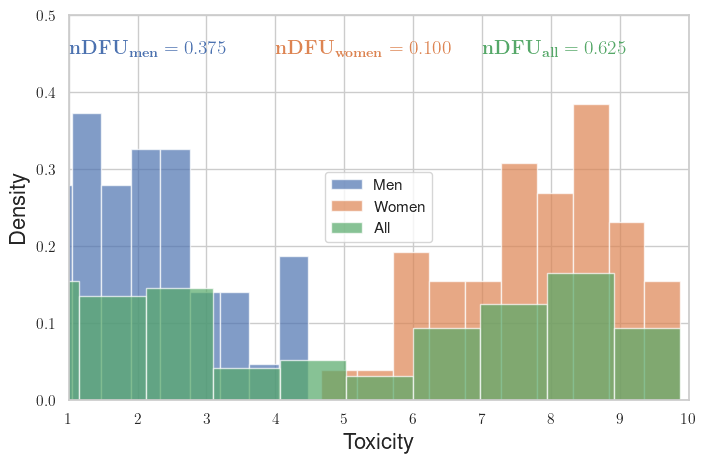
\includegraphics[width=0.8\linewidth]{ndfu_combined.png}
	\caption{Hypothetical example of a polarizing comment, where male and female annotators agree between themselves, but disagree with the opposite gender. Overall polarization ($nDFU_{all} = 0.625$) is much greater than the polarization exhibited by the annotations grouped by gender ($nDFU_{men} = 0.3725, nDFU_{women} = 0.1$).}
	\label{fig:ndfu_combined}
\end{figure}

\paragraph{Dataset polarization} Given this observation, we would be tempted to aggregate all annotations in the dataset and compare the polarization of each $\theta$ with the full set of annotations $A(c)$. However, this formulation would not work well. Figure~\ref{fig:ndfu_discussion} illustrates a hypothetical discussion with two comments, both of which are toxic, but where male and female annotators disagree on \emph{which} comment is the toxic one. If we aggregate the annotations to a single discussion, the opposing polarization effects might balance each other out, leading to a false negative. In simpler terms, polarization has a \textit{direction}, and care must be taken to not combine polarization effects of opposite directions.

In our example, while it is obvious that gender partly explains the polarization found in each of the individual comments ($nDFU_{all} \gg nDFU_{men}, nDFU_{all} \gg nDFU_{women}$), this observation is much harder to make when aggregating the two comments. This is graphically shown as the presence of three bimodal distributions instead of two unimodal distributions, and one bimodal (aggregated) distribution. To avoid this, we apply our statistic only on annotations that reference the same data-point.

\begin{figure*}
	\centering
    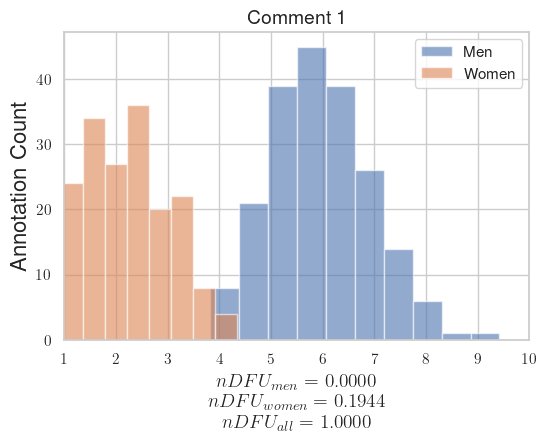
\includegraphics[width=0.3\linewidth]{ndfu_comment1.png}
    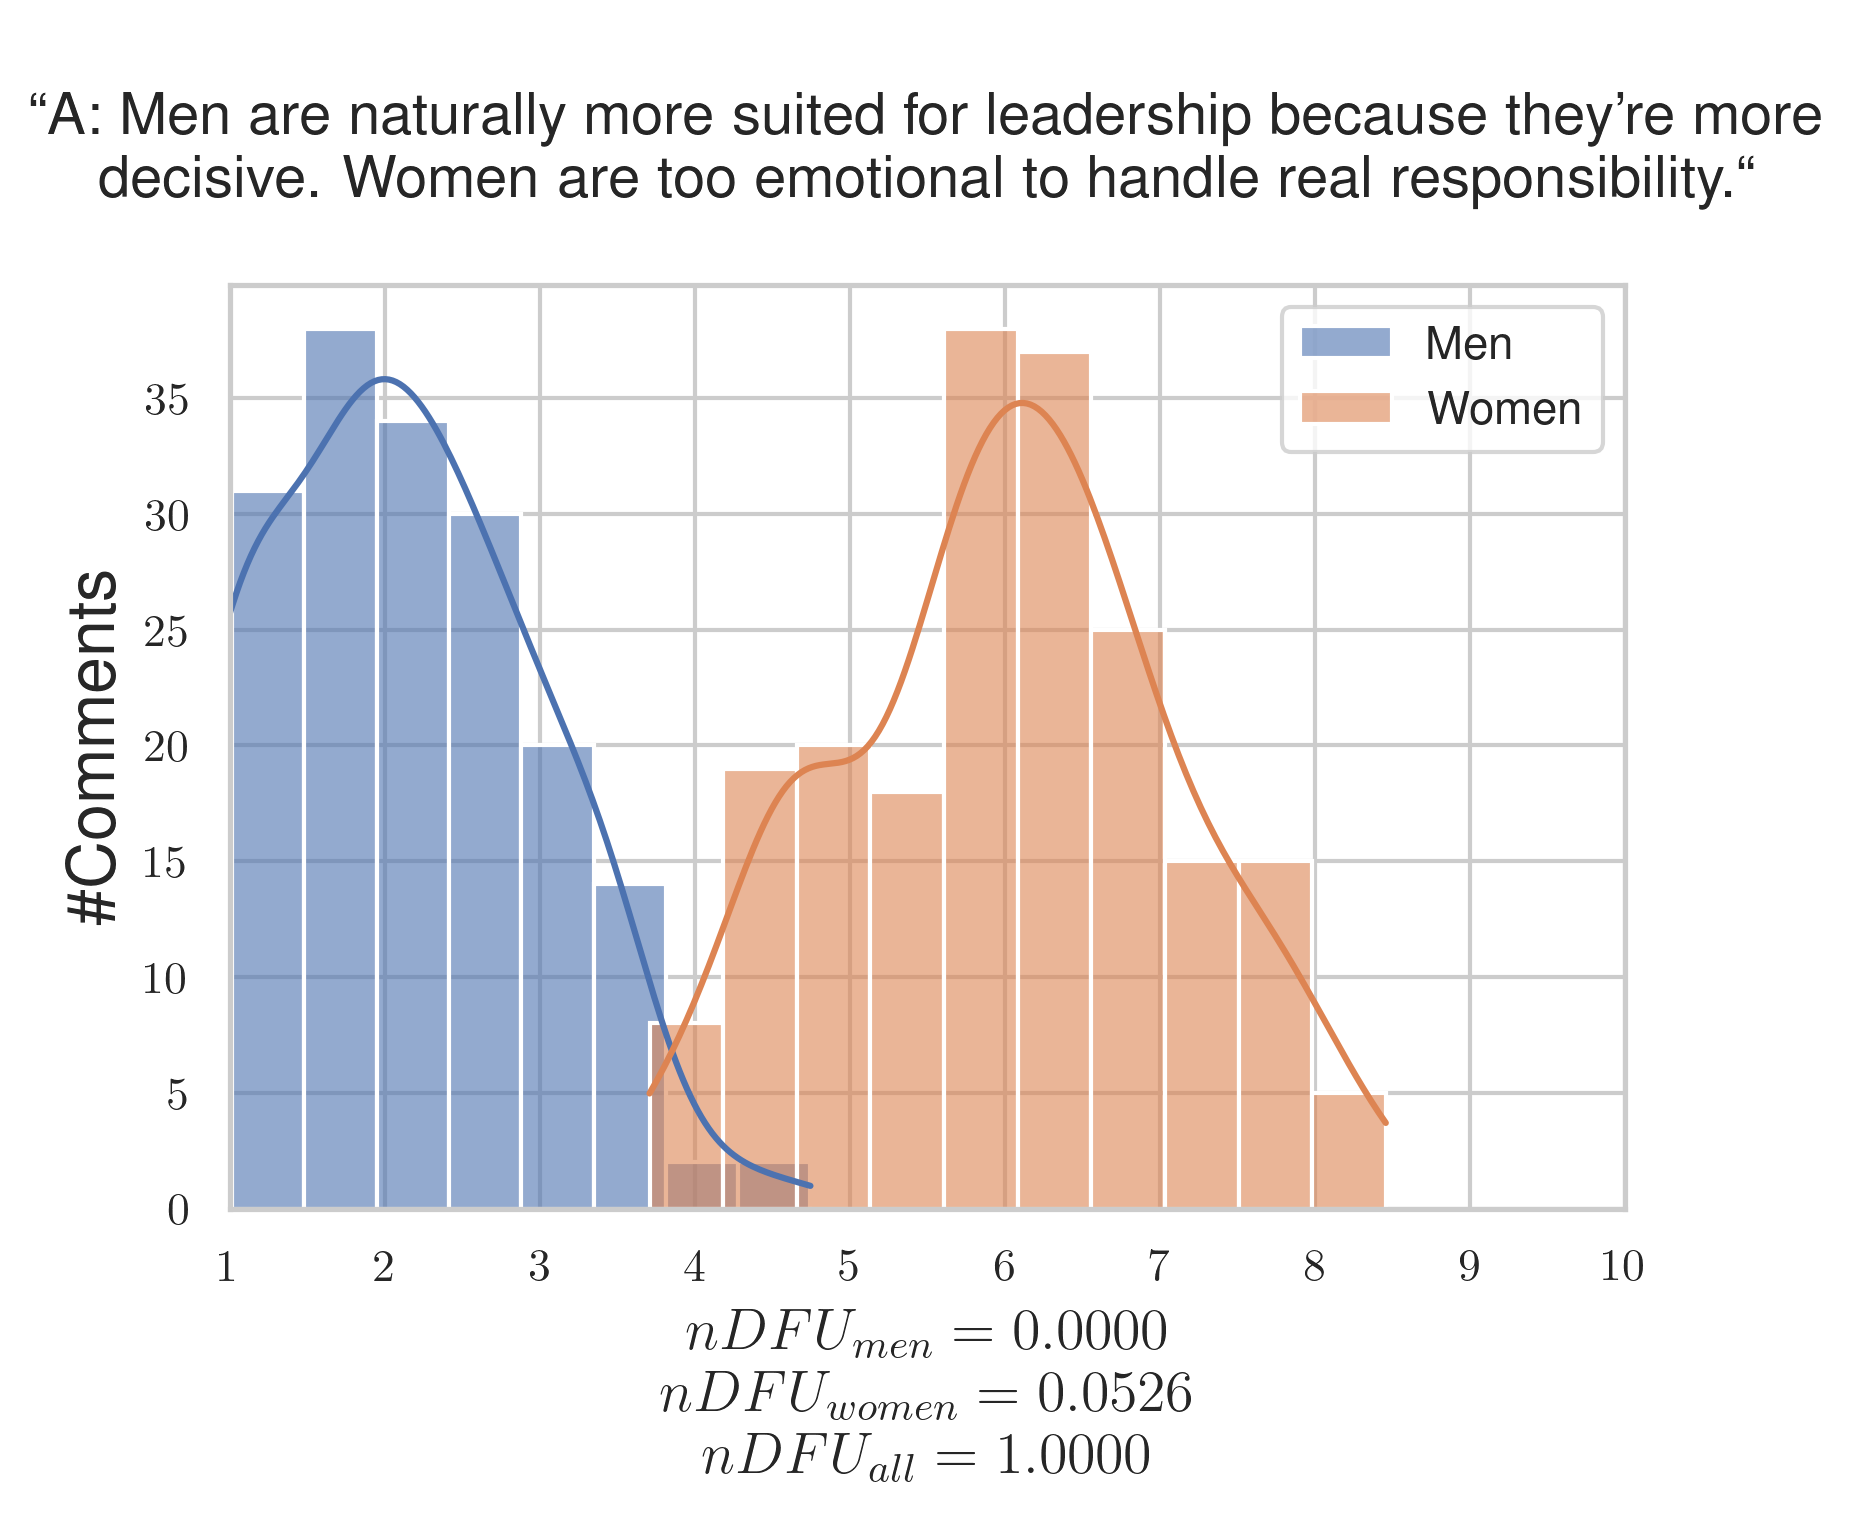
\includegraphics[width=0.3 \linewidth]{ndfu_comment2.png}
	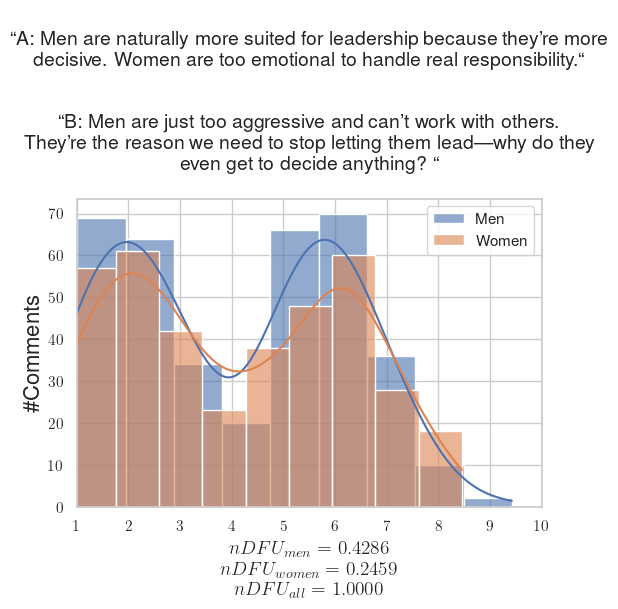
\includegraphics[width=0.3 \linewidth]{ndfu_discussion.png}
	\caption{Hypothetical example of a polarizing discussion with two comments, for which the annotators disagree on which is the toxic one. If we aggregate the two comments, the polarization scores for both men and women significantly rise, obscuring whether the exhibited polarization can be partially attributed to gender.}
	\label{fig:ndfu_discussion}
\end{figure*}

 
 
 \subsection{The pol-statistic}
 \label{ssec:methodology:polstat}
  
As demonstrated above, it is necessary to define a statistic for each individual data-point. We thus introduce the \textit{``pol-statistic''}, which quantifies the change in \ac{nDFU} when annotations are grouped by $\theta \in \Theta$.

In order to define this statistic, we need to measure (1) the polarization of a data-point when grouped by $\theta$, and (2) the ``inherent'' polarization present in the annotations, which is driven by either the contents of the data-point, or by the uncontrolled factors mentioned in \S\ref{ssec:methodology:problem}. Note that we can not directly compare the $\theta$-subset of annotations with the full set of annotations, since any statistical comparison between them violates the assumption of independent samples. %Removing the subset from the full set of annotations on the other hand, may introduce selection bias, especially when considering interactions between subgroups and confounding variables. % TODO: does this even make sense?

The observed polarization of a data-point on the group of annotations $\theta$ can be directly computed as: 
 \begin{equation}
 	pol(c, \theta) = nDFU(P(A(c), \theta)
 \end{equation}
 \noindent where $P(A(c), \theta_i) = \{a(c; \theta) \in A(c) | \theta=\theta_i\}$ is the partition of $A$ for a data-point $c$, for which its annotators belong to the \ac{SDB} group $\theta_i$.
 
 We can estimate the inherent polarization in data-point $c$ by bootstrapping. We randomly partition the data-point's annotations in $\lvert \Theta \rvert$ groups, with matching group sizes (e.g., if we have $100$ annotations, $80$ of which are made by male annotators and $20$ by female annotators, we will create random partitions of sizes $80$ and $20$). The randomly partitioned annotations are then sampled $t$ times. Formally, the expected inherent polarization will be given by:
 
 \begin{equation}
 	\label{eq:pol_expected}
 	\frac{1}{t} \sum_{i=1}^t  \textit{nDFU}(\tilde{P}_i(A(c)))
 \end{equation}
 \noindent where $\tilde{P}_i$ is the random partition operator with matching group sizes.


\subsection{Aposteriori Unimodality}
\label{ssec:methodology:aposteriori}

By obtaining the pol-statistics for all data-points in a dataset $d$ for \ac{SDB} $\theta$, we can get the mean observed polarization for the dataset:
\begin{equation}
	pol_{O}(d, \theta) = \frac{1}{\lvert d \rvert} \sum_{c \in d} (pol(c, \theta) - \frac{1}{t} \sum_{i=1}^t  \textit{nDFU}(\tilde{P}_i(A(c))))
\end{equation} 
\noindent and similarly the mean apriori dataset polarization:
\begin{equation}
	pol_{E}(d) = \frac{1}{\lvert d \rvert} \sum_{c \in d} \sum_{i=1}^t  \textit{nDFU}(\tilde{P}_i(A(c)))
\end{equation}

\noindent We can then define the Aposteriori Unimodality Statistic ($\kappa$) with a formulation inspired by Cohen's Kappa \cite{Cohen_1960}, as:
\begin{equation}
	\kappa = apunim(d, \theta) = \frac{pol_O(d, \theta) - pol_E(d)}{1 - pol_E(d)}
\end{equation}

The statistic is technically unbounded, but typically resides in the $[-1, 1]$ range. If $\kappa \approx 0$, the exhibited polarization among annotators of group $\theta$ does not surpass what would be expected by chance. If $\kappa > 0$, then the group partially explains a rise in polarization. Unlike Cohen's Kappa, the case of $\kappa < 0$ does have meaning; the group actually exhibits lower polarization compared to the whole. The scope of the statistic and its relationship with the previously presented statistics are demonstrated in Figure~\ref{fig::overview}. 

Like most metrics, we also include a p-value alongside the $\kappa$ value. This can be computed either non-parametrically, by repeatedly shuffling annotations and computing a null distribution of $apunim$, or parametrically, by assuming a normal distribution (which is generally a safe assumption if $t \geq 30$). %TODO: citation?
In the latter case, we compute:
 
\begin{equation}
	z = \frac{\hat{\kappa}  - \mathop{\mathbb{E}}[\kappa]}{SE(\hat{\kappa})}, p = 1 - \mathop{\Phi}(z)
\end{equation}

\begin{figure}
	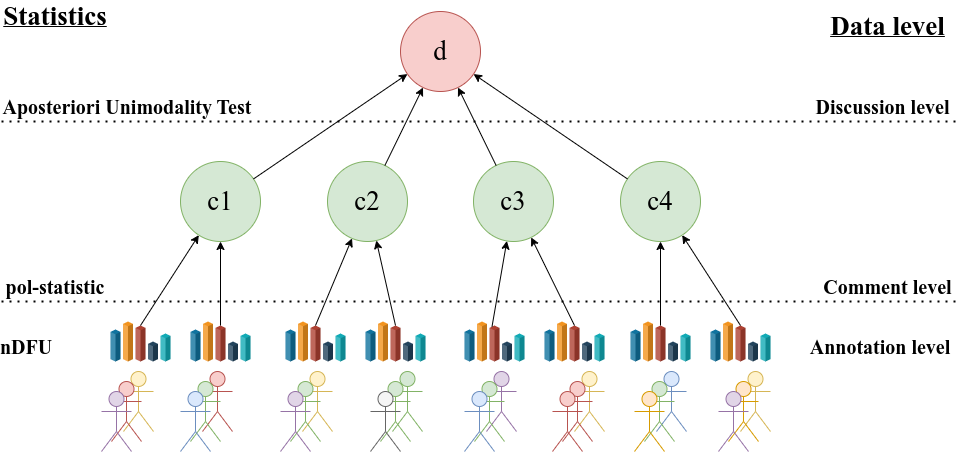
\includegraphics[width=\linewidth]{overview.png}
	\caption{An overview of the Aposteriori Unimodality Test. We gather statistical information from the annotations (different \acp{SDB} are denoted by different colors) via the \ac{nDFU} measure, which is aggregated on the data-point-level by the pol-statistic. The Aposteriori Unimodality Test is applied on the discussion level, operating on the pol-statistics of the individual data-points.}
	\label{fig::overview}
\end{figure}


\subsection{Technical Details}
\label{ssec:methodology:details}

Since we are simultaneously considering $\lvert \Theta \rvert$ hypotheses, we apply a multiple comparison correction to the resulting p-values. We choose the Holms method \parencite{holms}. The test is parameterized by the \ac{FWER}, which is used to tune the strength of the correction; we can increase this value to make our test more conservative towards multiple hypotheses \parencite{ChenFengYi2017}). In general, it is safe to set \ac{FWER} equal to the significance level of our test (e.g., $\textit{FWER} = 0.95$ if we are looking for $p < 0.05$).


\section{Results}
\label{sec:results}

We apply our test on four datasets; two human-annotated datasets, and two with comments and annotations generated by \acp{LLM}.

\subsection{Human Datasets}

We use the datasets provided by \textcite{kumar-et-al-2021} and \textcite{sap-etal-2022-annotators}. The datasets feature various online comments, each annotated by a number of human annotators ($5$ and $4-6$ annotators per comment respectively). The \textcite{sap-etal-2022-annotators} dataset includes racism annotations for $626$ Twitter/X comments, and standard \ac{SDB} information (age, race, education, gender). The \textcite{kumar-et-al-2021} dataset measures toxicity on various online comments, and the provided \acp{SDB} include mostly annotator experiences (e.g., whether they have been personally targeted online) as well as standard \ac{SDB} information such as sexual orientation, age and education. Since the dataset is extensive ($XXXX$ tweets), we only select a sample of $5000$ comments. This is due both to computational constraints, as well as statistical tests being unreliable on large enough samples \cite{trafimow2018manipulating}. Assuming a confidence level of $\alpha=0.05$ we test whether any of the provided \ac{SDB} dimensions can partially explain polarization in the toxicity/racism annotations. 

The results for the \textcite{kumar-et-al-2021} and \textcite{sap-etal-2022-annotators} datasets can be found in Tables~\ref{tab:res_kumar},~\ref{tab:res_kumar} respectively.

\begin{longtable}{llrr}
\caption{Aposteriori Unimodality kappa and pvalue results for the Sap et al. 2022 dataset} \label{tab:results_sap} \\
\toprule
 &  & kappa & pvalue \\
SDB Feature &  &  &  \\
\midrule
\endfirsthead
\caption[]{Aposteriori Unimodality kappa and pvalue results for the Sap et al. 2022 dataset} \\
\toprule
 &  & kappa & pvalue \\
SDB Feature &  &  &  \\
\midrule
\endhead
\midrule
\multicolumn{4}{r}{Continued on next page} \\
\midrule
\endfoot
\bottomrule
\endlastfoot
\multirow[t]{4}{*}{Age} & (-0.001, 20.0] & 0.000000 & 1.000000 \\
 & (20.0, 40.0] & -0.032111 & 0.819964 \\
 & (40.0, 60.0] & 0.036419 & 0.819964 \\
 & (60.0, 80.0] & 0.082569 & 0.819964 \\
\cline{1-4}
\multirow[t]{4}{*}{Ethnicity} & black & -0.415255 & 1.000000 \\
 & hisp & 0.000000 & 1.000000 \\
 & other & 0.000000 & 1.000000 \\
 & white & 0.147577 & 1.000000 \\
\cline{1-4}
\multirow[t]{3}{*}{Gender} & man & 0.151223 & 1.000000 \\
 & nonBinary & 0.000000 & 1.000000 \\
 & woman & -0.350066 & 1.000000 \\
\cline{1-4}
\end{longtable}

\begin{longtable}{llrr}
\caption{Aposteriori Unimodality kappa and pvalue results for the Kumar et al. 2021 dataset} \label{tab:results_kumar} \\
\toprule
 &  & kappa & pvalue \\
SDB Feature &  &  &  \\
\midrule
\endfirsthead
\caption[]{Aposteriori Unimodality kappa and pvalue results for the Kumar et al. 2021 dataset} \\
\toprule
 &  & kappa & pvalue \\
SDB Feature &  &  &  \\
\midrule
\endhead
\midrule
\multicolumn{4}{r}{Continued on next page} \\
\midrule
\endfoot
\bottomrule
\endlastfoot
\multirow[t]{7}{*}{Age} & 18 - 24 & 0.074931 & 0.636364 \\
 & 25 - 34 & 0.005710 & 0.636364 \\
 & 35 - 44 & 0.001821 & 0.636364 \\
 & 45 - 54 & -0.065202 & 0.636364 \\
 & 55 - 64 & -0.102204 & 0.636364 \\
 & 65 or older & -0.056338 & 0.636364 \\
 & Prefer not to say & 0.000000 & NaN \\
\cline{1-4}
\multirow[t]{9}{*}{Education} & Associate degree & -0.021541 & 1.000000 \\
 & Bachelor's degree & 0.011508 & 1.000000 \\
 & College, no degree & -0.121638 & 1.000000 \\
 & Doctoral degree & 0.000000 & 1.000000 \\
 & High School graduate & -0.009957 & 1.000000 \\
 & Master's degree & 0.216632 & 1.000000 \\
 & No high school & 0.000000 & 1.000000 \\
 & Prefer not to say & 0.000000 & 1.000000 \\
 & Professional degree & 0.000000 & 1.000000 \\
\cline{1-4}
\multirow[t]{2}{*}{Has Been Targeted} & False & -0.205239 & 0.683616 \\
 & True & 0.212707 & 0.683616 \\
\cline{1-4}
\multirow[t]{3}{*}{Is Parent} & No & -0.191852 & 0.677165 \\
 & Prefer not to say & 0.011125 & 0.333333 \\
 & Yes & 0.060523 & 0.677165 \\
\cline{1-4}
\multirow[t]{2}{*}{Is Transgender} & No & -0.282051 & 0.750000 \\
 & Yes & 1.000000 & 0.000000 \\
\cline{1-4}
\multirow[t]{5}{*}{Political Affiliation} & Conservative & 0.009239 & 0.615385 \\
 & Independent & -0.025947 & 0.615385 \\
 & Liberal & -0.022822 & 0.615385 \\
 & Other & 0.022005 & 0.384615 \\
 & Prefer not to say & 0.044586 & 0.615385 \\
\cline{1-4}
\multirow[t]{2}{*}{Seen Toxicity} & False & 0.133161 & 0.668966 \\
 & True & -0.180233 & 0.668966 \\
\cline{1-4}
\multirow[t]{5}{*}{Sexual Orientation} & Bisexual & 0.517556 & 0.936170 \\
 & Heterosexual & -0.364961 & 1.000000 \\
 & Homosexual & 0.015471 & 1.000000 \\
 & Prefer not to say & 0.000000 & 1.000000 \\
 & NaN & 0.000000 & NaN \\
\cline{1-4}
\multirow[t]{5}{*}{Thinks Religion Is Important} & Not important & -0.175184 & 0.812102 \\
 & Not too important & 0.035781 & 0.812102 \\
 & Prefer not to say & 0.000000 & 1.000000 \\
 & Somewhat important & 0.078472 & 0.812102 \\
 & Very important & 0.006711 & 0.812102 \\
\cline{1-4}
\multirow[t]{5}{*}{Thinks Toxicity Is Problem} & Frequently a problem & -0.007901 & 0.613333 \\
 & Not a problem & 0.123448 & 0.613333 \\
 & Occasionally a problem & -0.029524 & 0.613333 \\
 & Rarely a problem & 0.044052 & 0.613333 \\
 & Very frequently a problem & -0.009541 & 0.613333 \\
\cline{1-4}
\end{longtable}



\subsection{Synthetic Datasets}

We use two synthetic datasets; one is the \ac{VMD} presented in \textcite{tsirmpas2025scalableevaluationonlinefacilitation}. This dataset features $140$ discussions, each having $14$ comments (and usually up to $14$ facilitator comments), each comment annotated by 10 \ac{LLM} annotators, each supplied with a different \ac{SDB}. The second dataset, is an extension of \ac{VMD}, where we select four random unmoderated discussions, and employ 100 distinct \ac{LLM} annotators.

We find no statistically significant results in any of the \ac{SDB} dimensions, in any of the datasets (annotator age, gender, sexual orientation, education, employment and political alignment). While polarization does exist in the dataset, %TODO: show a graph of ndfu
it can not be attributed to any of the synthetic \ac{SDB} groups. This suggests that \ac{SDB} prompting can not be used to simulate annotations for human groups, which is consistent with relevant literature on the topic \parencite{anthis_2025,hewitt2024predicting,rossi_2024,jansen_2023,bisbee_2023,neumann_2025}.

The results for the \ac{VMD} and 100-annotator datasets can be found in Tables~\ref{tab:res_vmd},~\ref{tab:res_100} respectively.

\begin{longtable}{llrr}
\caption{Aposteriori Unimodality kappa and pvalue results for the 100 Annotator Synthetic dataset} \label{tab:results_100} \\
\toprule
 &  & kappa & pvalue \\
SDB Feature &  &  &  \\
\midrule
\endfirsthead
\caption[]{Aposteriori Unimodality kappa and pvalue results for the 100 Annotator Synthetic dataset} \\
\toprule
 &  & kappa & pvalue \\
SDB Feature &  &  &  \\
\midrule
\endhead
\midrule
\multicolumn{4}{r}{Continued on next page} \\
\midrule
\endfoot
\bottomrule
\endlastfoot
\multirow[t]{4}{*}{annot\_age} & (14.927, 33.25] & 0.074225 & 0.816667 \\
 & (33.25, 51.5] & 0.472547 & 0.816667 \\
 & (51.5, 69.75] & -0.829268 & 0.816667 \\
 & (69.75, 88.0] & -0.133195 & 0.816667 \\
\cline{1-4}
\multirow[t]{3}{*}{annot\_current\_employment} & blue-collar & -0.074895 & 0.816667 \\
 & unemployed & 0.580230 & 0.816667 \\
 & white-collar & -0.202996 & 0.816667 \\
\cline{1-4}
\multirow[t]{4}{*}{annot\_demographic\_group} & asian & 1.467547 & 0.816667 \\
 & black & 0.466443 & 0.816667 \\
 & other & -1.982043 & 0.816667 \\
 & white & 1.042252 & 0.816667 \\
\cline{1-4}
\multirow[t]{3}{*}{annot\_education\_level} & high-school & 0.916244 & 0.816667 \\
 & none & -1.021784 & 0.816667 \\
 & university & 0.366156 & 0.816667 \\
\cline{1-4}
\multirow[t]{3}{*}{annot\_politics} & apolitical & -1.844725 & 0.800000 \\
 & left-wing liberal & 1.058426 & 0.800000 \\
 & right-wing conservative & 0.664081 & 0.800000 \\
\cline{1-4}
\multirow[t]{3}{*}{annot\_sex} & female & -0.114674 & 0.800000 \\
 & male & -0.590249 & 0.800000 \\
 & non-binary & 3.545969 & 0.800000 \\
\cline{1-4}
\multirow[t]{4}{*}{annot\_sexual\_orientation} & bisexual & 2.554953 & 0.816667 \\
 & homosexual & -0.322894 & 0.816667 \\
 & other & -3.000413 & 0.816667 \\
 & straight & 0.303466 & 0.816667 \\
\cline{1-4}
\end{longtable}

\begin{longtable}{llrr}
\caption{Aposteriori Unimodality kappa and pvalue results for the Virtual Moderation Dataset dataset} \label{tab:results_virtual} \\
\toprule
 &  & kappa & pvalue \\
sdb_column &  &  &  \\
\midrule
\endfirsthead
\caption[]{Aposteriori Unimodality kappa and pvalue results for the Virtual Moderation Dataset dataset} \\
\toprule
 &  & kappa & pvalue \\
sdb_column &  &  &  \\
\midrule
\endhead
\midrule
\multicolumn{4}{r}{Continued on next page} \\
\midrule
\endfoot
\bottomrule
\endlastfoot
\multirow[t]{4}{*}{age_annot} & (20.956, 32.0] & 0.006954 & 0.651917 \\
 & (32.0, 43.0] & 0.045736 & 0.651917 \\
 & (43.0, 54.0] & 0.011376 & 0.651917 \\
 & (54.0, 65.0] & -0.042332 & 0.651917 \\
\cline{1-4}
\multirow[t]{11}{*}{current_employment_annot} & Botanist & 0.000000 & 1.000000 \\
 & Cybersecurity Expert & 0.000000 & 1.000000 \\
 & Farmer & 0.000000 & 1.000000 \\
 & Game Developer & 0.000000 & 1.000000 \\
 & Historian & 0.000000 & 1.000000 \\
 & Poet & 0.000000 & 1.000000 \\
 & Registered Nurse & 0.000000 & 1.000000 \\
 & Research Scientist & 0.000000 & 1.000000 \\
 & Retired Philosopher & 0.000000 & 1.000000 \\
 & Stock Trader & 0.000000 & 1.000000 \\
 & Travel Blogger & 0.000000 & 1.000000 \\
\cline{1-4}
\multirow[t]{5}{*}{education_level_annot} & Bachelor's & 0.016868 & 0.824760 \\
 & Master's & -0.014443 & 0.824760 \\
 & No formal education & 0.000000 & 1.000000 \\
 & PhD & -0.030773 & 0.824760 \\
 & Some College & 0.040793 & 0.824760 \\
\cline{1-4}
\multirow[t]{3}{*}{sex_annot} & female & 0.031136 & 0.993517 \\
 & male & -0.000060 & 0.993517 \\
 & non-binary & 0.000000 & 1.000000 \\
\cline{1-4}
\multirow[t]{6}{*}{sexual_orientation_annot} & Asexual & 0.000000 & 1.000000 \\
 & Bisexual & 0.000000 & 1.000000 \\
 & Heterosexual & -0.019488 & 1.000000 \\
 & Homosexual & 0.000000 & 1.000000 \\
 & Lesbian & 0.000000 & 1.000000 \\
 & Pansexual & 0.000000 & 1.000000 \\
\cline{1-4}
\end{longtable}



\subsection{Effect of number of annotators}
\label{ssec: results:num_annotators}

In \S\ref{ssec:methodology:aposteriori} we mentioned that the test relies on enough annotations for each \ac{SDB} group and data-point. This can be an issue, given the cost required to utilize multiple human annotators for each data-point \parencite{rossi_2024}. Figure~\ref{fig::std_error} demonstrates the effect of the number of annotators to the \textit{pol-statistic} estimation. We use the $100$-annotator synthetic dataset and sample progressively $3-100$ annotators with replacement, then calculate the standard error with the mean \textit{pol-statistic}. As expected, the standard error is inversely proportional to the number of annotators, although the difference is not great, even for a low number of annotators.

\begin{figure}
	
\includegraphics[width=\linewidth]{ndfu_std_error_sample_size.png}
	\caption{Standard error of the \textit{pol-statistic} when sampled with replacement from the $100$-annotator synthetic dataset for various number of annotators.}
	\label{fig::std_error}
\end{figure}


\section{Conclusion}

We introduced the ``Aposteriori Unimodality Test'', a statistical test that detects whether certain sociodemographic groups partly cause polarization in annotations. Our test is resistant to low samples of annotations, bypasses common statistical issues such as sample dependence, and avoids newly-discovered issues such as the presence of inherent polarization and polarization direction. We apply our test two human-generated and two \ac{LLM}-generated datasets and find interesting patterns on the former, and verify current literature on \ac{LLM} \ac{SDB} prompting on the latter.


\section{Limitations}

Since there are no other established tests that attribute polarization to sociodemographic characteristics, there is no way to verify that the results presented in \S\ref{sec:results} are accurate. Similarly, there is no qualitative way of evaluating our test, other than observations on the (non-) efficacy of \ac{LLM} {SDB} prompting and our own intuition. Lastly, while our test seems to work sufficiently well with a small number of annotators per data-point, we still encourage researchers using this test to have at least a few annotators of each sociodemographic group that is being tested, in their dataset.


\section{Ethical Considerations}

While our works aims to help protect marginalized and disadvantaged groups by attributing polarization to certain subgroups, it can be taken advantage of by malicious actors. Given a dataset with fine-grained \ac{SDB} information, these actors can use our test to target specific vulnerable groups. We thus urge researchers to keep datasets including such information protected, and provided to others only under explicit permission.

\printbibliography


\appendix
\section{Appendix}

\subsection{Acronyms}

\begin{acronym}[WWW]
    \acro{VMD}{Virtual Moderation Dataset}
    \acro{LLM}{Large Language Model}
    \acro{SDB}{SocioDemographic Background}
    \acro{nDFU}{normalized Distance From Unimodality}
	\acro{FWER}{Family-Wise Error Rate}
\end{acronym}


\subsection{Demonstrative examples}

Our paper uses synthetic examples to demonstrate the intuition behind the Aposteriori Unimodality test. These examples use random sampling of manually selected distributions. Table~\ref{tab:synthetic_annotation_sets} summarizes the synthetic annotation distributions used to demonstrate the Aposteriori Unimodality test. In each scenario, annotations for men and women were sampled independently from Gaussian distributions with distinct parameters.

\begin{table}[ht]
\centering
\begin{tabular}{|l|l|l|l|}
\hline
\textbf{Figure} & \textbf{Group} & \textbf{Distribution} & \textbf{Size} \\
\hline
Figure~\ref{fig:ndfu_combined}
  & $A_{men}$   & $\mathcal{N}(2, 1.3)$  & 50 \\
  & $A_{women}$ & $\mathcal{N}(8, 1.3)$  & 50 \\
\hline
Figure~\ref{fig:ndfu_discussion} (1st comment)
  & $A_{men}$   & $\mathcal{N}(6, 1)$  & 200 \\
  & $A_{women}$ & $\mathcal{N}(2, 1)$  & 200 \\
\hline
Figure~\ref{fig:ndfu_discussion} (2nd comment) 
  & $A_{men}$   & $\mathcal{N}(2, 1)$  & 200 \\
  & $A_{women}$ & $\mathcal{N}(6, 1)$  & 200 \\
\hline
\end{tabular}
\caption{Synthetic annotation sets used to illustrate the Aposteriori Unimodality test. Each group corresponds to samples drawn from a Gaussian distribution with specified mean and standard deviation.}
\label{tab:synthetic_annotation_sets}
\end{table}

\end{document}
